\documentclass{bmd2010p}

%\usepackage[colorlinks=true, linkcolor=blue]{hyperref}
\usepackage{graphicx}
\usepackage{subfiles}
\usepackage{subfig}

\begin{document}

\begin{center}
\fontsize{14}{20}{\bf Accurate Measurement of Bicycle Parameter[3pt]}
\end{center}

%%%%%%%%%%%%%%%% authors %%%%%%%%%%%%%%%
\begin{center}
\normalsize{\bf{Jason K. Moore$^{*}$, Mont Hubbard, A. L. Schwab$^\#$,
            J. D. G. Kooijman$^\dag$}}
\end{center}

\begin{center}
\begin{tabular}{c}
$^*$ Mechanical and Aerospace Engineering\\
University of California, Davis\\
One Shields Avenue, Davis, CA, 95616, USA\\
e-mail: jkmoor@ucdavis.edu, mhubbard@ucdavis.edu\\
\end{tabular}
\begin{tabular}{c}
$^\#$ Laboratory for Engineering Mechanics\\
Delft University of Technology\\
Mekelweg 2, 2628CD Delft, The Netherlands\\
e-mail: a.l.schwab@tudelft.nl, jodikooijman@gmail.com\\
\end{tabular} \\ \vspace{2.5ex}

\end{center}


\section*{ABSTRACT}
Accurate measurements of a bicycle's physical parameters are required for
realistic dynamic simulations and analysis. For the most basic models the
geometry, mass, mass location and mass distributions must be measured. More complex models
require measurements of tire characteristics, human characteristics, friction, stiffness, damping, etc. This
paper concerns the measurement of the minimal bicycle parameters required for
the benchmark bicycle presented in~\cite{Meijaard2007}. This
model is composed of four rigid bodies, has ideal rolling and frictionless joints,
and is assumed to be laterally symmetric. A set of 25
parameters is used to describe the geometry, mass, mass location and
mass distribution of each of the rigid bodies. The experimental methods
described herein are based primarily on the work
done in~\cite{Kooijman2006} but have been refined for improved accuracy and
methodology. Koojiman's work was preceded by \cite{Roland1971} who measured a bicycle in a
similar fashion and both~\cite{Dohring1953} and~\cite{Singh1971} who have used
similar techniques with scooters. We measured the characteristics of six
different bicycles, two of which were set up in two different configurations.
This is a total of eight different parameter sets that can be used with, but not
limited to, the benchmark bicycle model. The accuracy of all the measurements
are presented up through the eigenvalue prediction of the linear model and are
based on error propagation theory with correlations taken into account.

The six bicycles, chosen for both variety and convenience, are as follows:
\emph{Batavus Browser}, a Dutch style city bicycle measured with and without
instrumentation as described in~\cite{Kooijman2009a}; \emph{Batavus Stratos
Deluxe}, a Dutch style sporty city bicycle; \emph{Batavus Crescendo Deluxe} a
Dutch style city bicycle with a suspended fork; \emph{Gary Fisher Mountain
Bike}, a hardtail mountain bicycle; \emph{Bianchi Pista}, a modern steel frame
track racing bicycle; and \emph{Yellow Bicycle}, a stripped down aluminum frame
road bicycle measured in two configurations, the second with the fork rotated
in the headtube 180 degrees for larger trail.
\begin{keywords}
bicycle,
parameters,
eigenvalues,
Bode.
\end{keywords}

\section{INTRODUCTION}

This work is intended to document the indirect measurement of eight real
bicycles' physical parameters. The physical parameters measured are those that
are needed for the benchmark bicycle model~\cite{Meijaard2007}. The work is
based off of the techiques used to measure the instrumented bicycle in
\cite{Kooijman2006} and \cite{Kooijman2008}. I used the same techniques as
Kooijman to measure a second instrumented bicycle~\cite{Moore2009a}. This
method had low accuracy and the $I_{yy}$ moments of inertia were
not measured for the fork and frame. Furthermore, very little data exists on
the physical parameters of different types of bicycles and this work aims to
provide a small sample of bicycles.

D\"{o}hring measured the physical parameters of a scooter~\cite{Dohring1953}.
Singh and Goel measured the physical parameters of a scooter~\cite{Singh1971}.
Roland and Massing measured the physical parameters of a bicycle in much the
same was as presented, including calculations of uncertainty from the indirect
measurement techniques~\cite{Roland1971}. Patterson used a swing to measure the
inertia of a bicycle and rider~\cite{Patterson2004}. This work is based off of the work
done by Kooijman~\cite{Kooijman2006}. I worked with Jodi Kooijman for a year and
was able to use much of the same apparatus and refine the measurement
technique.

\section{Bicycle Descriptions}
\begin{description}
    \item[Batavus Browser]{The Batavus Browser is lower priced Dutch city bike.
        We measured the physical proprieties of the stock Browser model and
        also the same bike with the instrumentation used in our experiments.}
    \item[Batavus Crescendo Deluxe]{The Batavus Crescendo Deluxe is a
        contemporary of all-round cycling in cool black and white. A great bike
        for a good end to touring. And that works fine with 8 gears, suspension
        fork and suspension seatpost.}
    \item[Gary Fisher Mountain Bike]{The Gary Fisher Ziggurat is a modern front
        suspended mountain bike.}
    \item[2007 Bianchi Pista]{The Pista is a modern steel track bicycle.}
    \item[Batavus Stratos Deluxe]{Is a Dutch sport bicycle.}
    \item[Yellow Bicycle]{The yellow is a bicycle used in the lab to
        demonstrate that a bicycle is stable at certain speeds. It is an
        aluminum road frame of unknown make with the majority of components
        removed. The wheels, drop handlebar, seat, seat post and bottom bracket
        are the only parts on the bike. The fork has been reversed to
        ''increase``~\cite{Kooijman2006} the stability of the bicycle. The
        bicycle was measured with both the fork in normal position and the fork
        reversed.}
\end{description}
\begin{figure}[htbp]
    \centering
    \subfloat[Batavus Browser]{
        \label{fig:browser}\includegraphics[width=1.75in]{../../../images/browserIns_sub.jpg}}
    \subfloat[Batavus Crescendo Deluxe]{
        \label{fig:crescendo}\includegraphics[width=1.75in]{../../../images/crescendo_sub.jpg}}
    \subfloat[Gary Fisher]{
        \label{fig:fisher}\includegraphics[width=1.75in]{../../../images/fisher_sub.jpg}}
        \\
    \subfloat[Bianchi Pista]{
        \label{fig:pista}\includegraphics[width=1.75in]{../../../images/pista_sub.jpg}}
    \subfloat[Batavus Stratos Deluxe]{
        \label{fig:stratos}\includegraphics[width=1.75in]{../../../images/stratos_sub.jpg}}
    \subfloat[Yellow Bicycle]{
        \label{fig:yellow}\includegraphics[width=1.75in]{../../../images/yellow_sub.jpg}}
    \caption{The six bicycles measured in the experiments. The Batavus
    Browser~\subref{fig:browser} is shown with the instrumentation and the
    Yellow Bicycle~\subref{fig:yellow} is shown with its fork reversed.}
    \label{fig:bicycles}
\end{figure}
\section{Accuracy}
Error propagation theory was utilized to calculate what the accuracy the
benchmark ideal parameters are based on the measurements taken. If $x$ is a
random variable and is defined as $x=f(u,v,\ldots)$ then the sample variance of
$x$ is defined as
\begin{equation}
    s_x^2 = \frac{1}{N-1}\sum^N_{i=1}
    \left[(u_i - \bar{u})^2\left(\frac{\partial x}{\partial u}\right)^2 +
    (v_i - \bar{v})^2\left(\frac{\partial x}{\partial v}\right)^2 +
    2(u_i - \bar{u})(v_i - \bar{v})\left(\frac{\partial x}{\partial u}\right)\left(\frac{\partial x}{\partial v}\right)
    + \ldots\right]
    \label{eqn:sampleVariance}
\end{equation}
Using the definitions for variance and covariance
Equation~\ref{eqn:sampleVariance} can be simplified to
\begin{equation}
    s_x^2 = s_u^2\left(\frac{\partial x}{\partial u}\right)^2 +
            s_v^2\left(\frac{\partial x}{\partial v}\right)^2 +
            2s_{uv}\left(\frac{\partial x}{\partial u}\right)\left(\frac{\partial x}{\partial v}\right)
            + \ldots
    \label{eqn:variance}
\end{equation}
If $u$ and $v$ are uncorrelated then $s_{uv}=0$. We assume that the all the
random variables hereafter are uncorrelated. Equation~\ref{eqn:variance} can be
used to calculated the variance of all types of functions. The most basic are
functions such as addtion
\begin{eqnarray}
    \label{eqn:addition}
    x &=&  au + bv\\
    s_x &=& a^2s_u^2 + b^2s_v^2
\end{eqnarray}

\section{Geometry}

\subsection{Wheel radius}
The radius of the front $r_\mathrm{F}$ and rear $r_\mathrm{R}$ wheels were
measured by measuring the linear distance traversed along the ground through
either 13 or 14 rotations of the wheel. Each wheel was measured separately and
the measurements were taken with a 72kg rider seated on the bicycle. A 30 meter
tape measure (resolution: 2mm) was taped on a flat level smooth floor. The tire
was marked with chalk and aligned with the tape measure. The accuracy of the
distance measurement is approximately $\pm0.005$m. The tires were pumped to the
recommended inflation pressure before the measurements. The wheel radius is
calculated by
\begin{equation}
	r=\frac{\textrm{distance}}{2\cdot\pi\cdot\textrm{rotations}}
	\label{eq:wheelRadius}
\end{equation}
\begin{equation}
    \sigma_r^{2}=\left(\frac{\sigma_d}{2\pi n}\right)^{2}
    \label{eq:WheelRadVar}
\end{equation}
\begin{figure}[tb]
	\begin{center}
		\includegraphics[width=4in]{../../../images/tireChalk.jpg}
	\end{center}
	\caption{Wheel and tire with chalk mark aligned to the tape measure.}
	\label{fig:tireChalk}
\end{figure}
\begin{table}
	\begin{tabular}{llllllll}
	Bicycle   & B      & B*     & C      & G      & P      & S      & Y \& Y*\\
    \hline
	Front\\
	Pressure  & 3.5    & 3.5    & 4      & 4      & 6.9    & 4.5    & 4      \\
	Distance  & 28.060 & 27.980 & 27.980 & 29.044 & 29.366 & 27.772 & 27.925 \\
	Rotations & 13     & 13     & 13     & 14     & 14     & 13     & 13     \\
	Radius    & 0.344  & 0.343  & 0.343  & 0.330  & 0.334  & 0.340  & 0.342  \\
	Rear\\
	Pressure  & 3.5    & 3.5    & 4      & 4      & 6.9    & 4.5    & 3.5    \\
	Distance  & 27.850 & 27.835 & 27.768 & 29.788 & 29.212 & 29.774 & 27.884 \\
	Rotations & 13     & 13     & 13     & 14     & 14     & 14     & 13     \\
	Radius    & 0.341  & 0.341  & 0.340  & 0.339  & 0.332  & 0.338  & 0.341
	\end{tabular}
	\caption{}
	\label{tab:wheelRadius}
\end{table}
\subsection{Head tube angle}
The head tube angle was measured directly using an electronic level with a
$\pm0.2^{\circ}$ accuracy. The bicycle was fixed vertically, the front wheel
was aligned with the rear frame and the bicycle was unloaded. The steer axis
tilt $\lambda$ is the complement to the head tube angle.
\begin{equation}
    \lambda=\frac{\pi}{180^{\circ}}(90^{\circ}-\lambda_{ht})
\label{eq:headTubeAngle}
\end{equation}
\begin{equation}
    \sigma_\lambda^{2}=-\sigma_{\lambda_{ht}}^{2}\left(\frac{\pi}{180^\circ}\right)^2
    \label{eq:HeadTubeAngleVar}
\end{equation}
\begin{table}
	\begin{tabular}{lllllllll}
    \hline
	Bicycle   & B      & B*     & C      & G      & P      & S      & Y      & Y*\\
	Head tube angle & 67.1 & 67.1 & 69.0 & 71.1 & 74.2 & 73.1 & 72.7 & 70.6\\
	Steer axis tilt & 0.400 & 0.400 & 0.367 & 0.330 & 0.276 & 0.295 & 0.302 & 0.339
	\end{tabular}
	\caption{Head tube angle and steer axis tilt}
	\label{tab:lambda}
\end{table}

\subsection{Trail}
Trail is difficult to measure directly so we instead chose to measure the fork
offset. The fork offset was measured by clamping the steer tube of the front
fork into a v-block on a flat table. A ruler was used to measure the height of
the center of the head tube and the height of the center of the axle axis. The
fork blades where aligned such that the axle axis was parallel to the table
surface.
\begin{equation}
	c=\frac{r_\mathrm{F}\sin{\lambda}-f_o}{\cos{\lambda}}
	\label{eq:trail}
\end{equation}
\begin{equation}
    \sigma_{c}^{2}=\sigma_{r_{\mathrm{F}}}^{2}\tan^2{\lambda} -
    \sigma_{f_o}^{2}\sec^2{\lambda} +
    \sigma_{\lambda}^{2}\left(r_\mathrm{F}\sec^2{\lambda} -
    f_o\sec{\lambda}\tan{\lambda}\right)^2
    \label{eq:TrailVar}
\end{equation}
\begin{table}
	\begin{tabular}{lllllllll}
	Bicycle     & B     & B*    & C     & G     & P     & S     & Y     & Y*\\
    \hline
	Fork offset & 0.071 & 0.071 & 0.045 & 0.039 & 0.032 & 0.045 & 0.057 & -0.057\\
	Trail       & 0.069 & 0.068 & 0.083 & 0.072 & 0.062 & 0.056 & 0.047 & 0.180
	\end{tabular}
	\caption{Head tube angle and steer axis tilt}
	\label{tab:trail}
\end{table}
\subsection{Wheelbase}
The wheelbase was measured directly using a tape measure while the bicycle was
in the same upright fixed position used when measuring the head tube angle.
\begin{table}
	\begin{tabular}{lllllllll}
	Bicycle    & B     & B*    & C     & G     & P     & S     & Y     & Y*\\
    \hline
	Wheel base & 1.121 & 1.121 & 1.101 & 1.070 & 0.989 & 1.037 & 1.089 & 0.985
	\end{tabular}
	\caption{Wheelbase values.}
	\label{tab:wheelbase}
\end{table}

\section{Mass}
The total mass of each bicycle was measured using a spring scale with a
resolution of 100g. Then each of the four bicycle parts were measured using a
Molen 20kg scale with a resolution of 20g.
\begin{figure}[htbp]
    \begin{center}
        \includegraphics[width=4in]{../../../images/massScale.jpg}
    \end{center}
    \caption{The scale used to measure the mass of each bicycle component.}
    \label{fig:massScale}
\end{figure}
\begin{table}
    \centering
	\begin{tabular}{llllllllll}
		Bicycle &     $\sigma_m$ & B     & B*    & C     & G     & P    & S     & Y     & Y*\\
        \hline
		total   &    0.1       & 18.5  & 23.5  & 20.9  & 10.5  & 9.9  & 17.6  & 10.2  & 10.2\\
        \hline
		frame   &    0.02      & 9.86  & 14.71 & 9.18  & 4.48  & 4.49 & 7.22  & 3.31  & 3.31\\
		fork    &    0.02      & 3.22  & 3.22  & 4.57  & 2.52  & 2.27 & 3.04  & 2.45  & 2.45\\
		rear wheel & 0.02      & 3.11  & 3.11  & 3.96  & 1.94  & 1.38 & 3.96  & 2.57  & 2.57\\
		front wheel& 0.02      & 2.02  & 2.02  & 3.55  & 1.50  & 1.58 & 3.33  & 1.90  & 1.90\\
		total sum  & 0.04      & 18.21 & 23.06 & 21.26 & 10.44 & 9.72 & 17.55 & 10.23 & 10.23
	\end{tabular}
	\caption{Mass of bicycles and parts}
	\label{tab:mass}
\end{table}
\section{Center of Mass}
\subsection{Wheels}
The centers of mass of the wheels are assumed to be at their geometrical centers.
\subsection{Rear frame}
The rear frame was hung in three orientations as a torsional pendulum (the
pendulum was used to measure moments of inertia). I
assumed that the frame was laterally symmetric. The
frame could rotate about a joint such that gravity aligned the center of mass
with the pendulum axis. The orientation angle of the headtube $\alpha$
Figure~\ref{fig:angles} relative
to the earth was
measured using the digital level Figure~\ref{fig:level}. A string was aligned with the pendulum axis
and allowed to pass by the frame. The horizontal distance $a_\mathrm{B}$ between the rear
axle and the string (CoM line) was measured by aligning a ruler perpendicular to
the string. The distance $a$ was negative if the string fell to the right of
the rear axle and positive if it fell to the left of the rear axle. These
measurements allow for the calculation of the center of mass location in the
global reference frame.
\begin{figure}[htbp]
    \begin{center}
        \includegraphics[width=4in]{../../../images/pendDist.jpg}
    \end{center}
    \caption{Measuring the distance from the pendulum axis to the rear wheel
    axle using level ruler.}
    \label{fig:PendDist}
\end{figure}
\begin{figure}[tb]
	\begin{center}
		\includegraphics[width=4in]{../../../images/level.jpg}
	\end{center}
	\caption{The digital level was mounted to a straight edge that was aligned
    with the headtube of the bicycle frame. This was done without allowing the
    straight edge to touch the frame. The frame wasn't completely stationary so
    this was difficult. The light frame oscillations could be damped out by
    submerging a low hanging area of the frame into a bucket of water to
    decrease the oscillation.}
	\label{fig:level}
\end{figure}
The frame rotation angle $\beta$ is defined as rotation of the frame in the
nominal configuration to the hanging orientation, rotated about the $Y$ axis.
\begin{figure}[tb]
	\begin{center}
		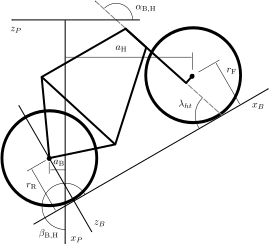
\includegraphics[width=4in]{../../../figures/angles.pdf}
	\end{center}
	\caption{Pictorial description of the angles and dimensions that related
    the nominal bicycle reference frame $XYZ_B$ with the pendulum reference frame
    $XYZ_P$.}
	\label{fig:angles}
\end{figure}
\begin{equation}
	\beta=\lambda-\alpha
    \label{eq:frameRotAng}
\end{equation}
\begin{equation}
    \sigma_{\beta}^{2} = \sigma_{\lambda}^{2} + \sigma_{\alpha}^{2}
    \label{eq:FrameRotAngVar}
\end{equation}
The pendulum axis $X_P$ is simply a line in the nominal bicycle reference frame with a slope $m$ and a z-intercept $b$. The slope can be shown to be
\begin{equation}
	m_i=-\tan{\beta_i}
\label{eq:slope}
\end{equation}
\begin{equation}
    \sigma_{m}^{2} = \sigma_{\beta}^{2}\sec^{4}{\beta}
    \label{eq:SlopeVar}
\end{equation}
The z-intercept can be shown to be
\begin{equation}
    b_i=-\left(\frac{a_\mathrm{B}}{\cos{\beta_i}}+r_\mathrm{R}\right)
    \label{eq:zInt}
\end{equation}
\begin{equation}
    \sigma_{b}^{2} = \sigma_{a}^{2}\sec^{2}{\beta} +
    \sigma_{r_\mathrm{R}}^{2} +
    \sigma_{\beta}^{2}a^{2}\sec^{2}{\beta}\tan^{2}{\beta}
    \label{eq:zIntvar}
\end{equation}
Only two lines are required to calculate the center of mass of the laterally
symmetric frame, but more orientations increase the center of mass measurement
accuracy. The three lines are defined as:
\begin{equation}
   y = m_ix+b_i
   \label{eq:line}
\end{equation}
The CoM location can be calculated by finding the intersection of these three
lines. Two approaches were used used to calculate the center of mass. Intuition
leads me to think that the center of mass is located at the centroid of the
triangle made by the three intersecting lines. The centroid can be found by
calculating the intersection point of each pair of lines and then averaging the
three intersection points.
\begin{figure}[htpb]
    \begin{center}
        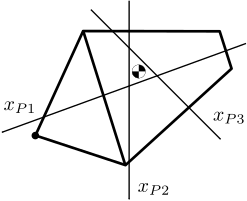
\includegraphics{../../../figures/triangle.pdf}
    \end{center}
    \caption{Exaggerated intersection of the three pendulum axes and the
    location of the center of mass.}
    \label{fig:triangle}
\end{figure}
\begin{equation}
	\left[
	\begin{array}{cc}
		-m_1 & 1\\
		-m_2 & 1
	\end{array}
	\right]
	\left[
	\begin{array}{c}
		x_a\\
		z_a
	\end{array}
	\right]
	=
	\left[
	\begin{array}{c}
		b_1\\
		b_2
	\end{array}
	\right]
\label{eq:linearSystem}
\end{equation}
\begin{equation}
    x_\mathrm{B} = \frac{x_a + x_b + x_c}{3}
\end{equation}
\begin{equation}
    z_\mathrm{B} = \frac{z_a + z_b + z_c}{3}
\end{equation}
Alternatively the three lines can be treated as an over determined linear
system and the least squares method is used to find a unique solution. This
solution is not at the centroid of the triangle made by the intersecting lines.
I am not sure which solution is theoretically the correct one for the location
of the center of mass.
\begin{equation}
	\left[
	\begin{array}{cc}
		-m_1 & 1\\
		-m_2 & 1\\
		-m_3 & 1
	\end{array}
	\right]
	\left[
	\begin{array}{c}
        x_\mathrm{B}\\
        z_\mathrm{B}
	\end{array}
	\right]
	=
	\left[
	\begin{array}{c}
		b_1\\
		b_2\\
		b_3
	\end{array}
	\right]	
\label{eq:leastSquares}
\end{equation}
\subsection{Fork}
The fork and handlebars are a bit trickier to hang in three different
orientations. Typically two angles can be obtained by clamping to the steer
tube at the top and the bottom. The third angle can be obtained by clamping to
the stem. The center of mass of the fork is calculated in the same fashion. The
slope of the line in the benchmark reference frame is the same as for the
frame but the z-intercept is different:
\begin{equation}
    b = w\tan{\beta} - r_\mathrm{F} - \frac{a}{\cos{\beta}} 
    \label{eq:zIntFork}
\end{equation}
\begin{equation}
    \sigma_{b}^{2} = \sigma_{w}^{2}\tan^{2}\beta +
    \sigma_{\beta}^{2}\left(w\sec^{2}\beta -
    a\sec\beta\tan\beta\right)^{2} + \sigma_{r_\mathrm{F}}^{2} +
    \sigma_{a}^{2}\sec^{2}\beta
    \label{eq:zIntForkVar}
\end{equation}
\section{Moment of Inertia}
The moments of inertia of the wheels, frame and fork were measured by taking
advantage of the assumed symmetry of the parts and by hanging the parts as both
compound and torsional pendulums and measuring their period of oscillation when
perturb at small angles. The rate of oscillation was measured was measured
using a \href{http://www.siliconsensing.com/CRS03}{Silicon Sensing CRS03 100
deg/s rate gyro}. The rate gyro was sampled at
1000hz with a
\href{http://sine.ni.com/nips/cds/view/p/lang/en/nid/14604}{National
Instruments USB-6008 12 bit data acquisition unit} and
Matlab. The measurement duration were either 15 or 30 secs and each moment of
inertia measurement was performed three times. No extra care was taken to
calibrate the rate gyro, maintain a constant power source (i.e. the battery
drains slowly), or account for drift. The raw voltage signal was used to
determine only the period of oscillation which is need for the moment of inertia
calculations.
\begin{figure}[tbp]
    \begin{center}
        \includegraphics[width=4in]{../../../plots/PendFit/BrowserFrameCompoundFirst1.png}
    \end{center}
    \caption{Example of the raw voltage data taken during a 30 second
    measurement of the oscillation of one of the components.}
    \label{fig:voltage}
\end{figure}
The following function Eqn~\ref{eqn:decayOs} was fit to the data using a nonlinear least squares fit
routine for each experiment.
\begin{equation}
    f(t) = A + e^{-\zeta\omega t}\left[B\sin{\sqrt{1-\zeta^2}\omega t} +
    C\cos{\sqrt{1-\zeta^2}\omega t}\right]
    \label{eqn:decayOs}
\end{equation}
Most of the data fit the damped oscillation function well with very light (and
ignorable) damping. There were several instances of beating-like phenomena for
some of the parts at particular orientations. Roland and
Massing~\cite{Roland1971} also encountered this problem and used a bearing to
prevent the torsional pendulum from swinging. Figure~\ref{fig:beating} shows an
example of the beating like phenomena.
\begin{figure}[htpb]
    \begin{center}
        \includegraphics[width=4in]{../../../plots/PendFit/CrescendoForkTorsionalFirst2.png}
    \end{center}
    \caption{An example of the beating-like phenomena observed on 5\% of the
    experiments.}
    \label{fig:beating}
\end{figure}
The physical phenomena that was observed for data sets such as these were that
the bicycle frame or fork was perturbed torsionally. After set into motion the
torsional motion died out and a longitudinal swinging motion increased. The
motions alternated back and forth with neither ever reaching zero. The
frequencies of these motions were very close to one another and it is not
apparent how dissect the two. We explored fitting to a function such as
\begin{equation}
    f(t) = A\sin{(\omega_1 t)} + B\sin{(\omega_2 t + \phi)} + C
    \label{eqn:sumSines}
\end{equation}
But the fit predicts that $\omega_1$ and $\omega_2$ have very similar
frequencies. There was no easy way to choose which of the two $\omega$'s was
the one associated with the torsional oscillation. Some work was done to model
the torsional pendulum as a laterally flexible beam to determine this, but we
thought the improvement in the accuracy of the period calculation would not
improve enough for the effort required. Future experiments should simply
prevent the swinging motion of the pendulum without damping the torsional
motion. Roland and Massing~\cite{Roland1971} noted that they had this same problem and solved it
by hold the torsional rod in a fixed bearing.

The period for a damped oscillation is
\begin{equation}
    T = \frac{2\pi}{\sqrt{1-\zeta^2}\omega_n}
    \label{eqn:periodDamped}
\end{equation}
and for light damping
\begin{equation}
    T \approx \frac{2\pi}{\omega_n}
    \label{eqn:period}
\end{equation}
The uncertainty in the period, $T$, can be determined from the fit. Firstly,
the variance of the fit is
\begin{equation}
    \sigma_y^2 =
    \frac{1}{N-5}\sum_{i=1}^N(y_{mi}-\bar{y}_m)^2-(y_{pi}-\bar{y}_m)^2
    \label{eqn:fitVariance}
\end{equation}
The covariance matrix of the fit function can be formed
\begin{equation}
    \mathbf{U} = \sigma_y^2\mathbf{H}^{-1}
    \label{eqn:covariance}
\end{equation}
where $\mathbf{H}$ is the Hessian~\cite{Hubbard1989b}. $\mathbf{U}$ is a $5\times5$ matrix with the
variances of each of the five fit parameters along the diagonal. This assumes
that the parameters are uncorrelated [note for Jason: you may have to take into
account correlation for this..maybe checkout the R function for nls]. The
variance of $T$ can be computed using the variance of $\zeta$ and $\omega$. It
is important to note that the uncertainties in the period are very low
($<10e-4$), even for the fits with low $r^2$ values due to the beating issue.
\subsection{Torsional Pendulum}
A torsional pendulum was used to measure all of moments of inertia about axes
in the lateral symmetric plane of each of the wheels, fork and frame. The
pendulum is made up of a rigid mount, an upper clamp, a torsion rod, and
various lower clamps.
\begin{figure}[htbp]
    \begin{center}
        \includegraphics[width=4in]{../../../images/fixture.jpg}
    \end{center}
    \caption{The rigid pendulumfixture mounted to a concrete column.}
    \label{fig:fixture}
\end{figure}
A 5mm diameter, 1m long mild steel rod was used as the torsion
spring. A lightweight, low relative moment of inertia clamp was constructed
that could clamp the rim and the tire. The wheel was hung freely such that the
center of mass aligned with the torsional pendulum axis and then it was
secured. The wheel was then perturbed and it oscillated about the pendulum axis.
The rate gyro was mounted on the clamp in line with the pendulum axis. The
radial moment of inertia can can calculated as such:

The torsional pendulum was calibrated using a known moment of inertia. 
\begin{figure}[htbp]
    \begin{center}
        \includegraphics[width=4in]{../../../images/rod.jpg}
    \end{center}
    \caption{The steel calibration rod.}
    \label{fig:rod}
\end{figure}
A torsional pendulum almost identical to the one used in
\cite{Kooijman2006} was used to measure the averaged period $\overline{T}_i$ of
oscillation of the rear frame at three different
orientation angles $\beta_i$, where $i=1$, $2$, $3$, as shown in
Fig.~\ref{fig:triangle}. The parts were perturbed lightly, less than 1 degree,
and allowed to oscillate about the pendulum axis through at least ten periods.
The time of oscillation was recorded via a stopwatch ($\pm1$~s). This was done
three times for each frame and the recorded times were averaged. The
coefficient of elasticity $k$ for the torsional pendulum had previously been
measured in \cite{Kooijman2006} and found to be $k=5.01\pm0.01$
$\frac{\textrm{Nm}}{\textrm{rad}}$.

\subsection{Wheels}
The wheels are assumed to be symmetric laterally and about any radial axis. Thus only two
moment's of inertia are required. The moment of inertia about the axle was
measured by hanging the wheel as a compound pendulum. The wheel was hung on a
horizontal rod and perturbed to oscillate about the axis of the rod. This rate
gyro was attached to the spokes near the hub and orientated mostly along the
axle axis. The wheels tended to precess at the contact point about the vertical
axis. This adds a very low frequency component of rate along the vertical axis,
but should not affect the compound pendulum axis. A better fixture for the
wheel could prevent the precession. The pendulum arm length is the distance
from the rod/rim contact point to the mass center of the wheel. The inner
diameter of the rim was measured and divided by two to get $l$. The moment of
inertia about the axle is calculated by:
\begin{equation}
    I_{\mathrm{R}yy} = \left(\frac{\bar{T}}{2\pi}\right)^2m_\mathrm{R}gl_\mathrm{R} -
    m_\mathrm{R}l^2
\end{equation}
\begin{figure}[htbp]
    \begin{center}
        \includegraphics[width=4in]{../../../images/CrescendoFwheelTorsionalFirst.jpg}
    \end{center}
    \caption{The front wheel of the Crescendo hung as a torsional pendulum.}
    \label{fig:FwheelTor}
\end{figure}
The radial moment of inertia was measured by hanging the wheel as a torsional
pendulum. A 5mm diameter, 1m long mild steel rod was used as the torsion
spring. A lightweight, low relative moment of inertia clamp was constructed
that could clamp the rim and the tire. The wheel was hung freely such that the
center of mass aligned with the torsional pendulum axis and then it was
secured. The wheel was then perturbed and it oscillated about the pendulum axis.
The rate gyro was mounted on the clamp in line with the pendulum axis. The
radial moment of inertia can can calculated as such:
\begin{equation}
    I_{xx} = \frac{k\bar{T}^2}{4\pi^2}
\end{equation}
Finding the inertia tensors of the wheels is less complex because the wheels
are symmetric about three orthogonal planes so there are no products of
inertia. The $I_{xx}=I_{zz}$ moments of inertia were calculated by measuring
the averaged period of oscillation about an axis in the $XZ$-plane using the
torsional pendulum setup and Eq.~\ref{eq:torPend}. The $I_{yy}$ moment of
inertia was calculated with a compound pendulum as described in
\cite{Kooijman2006} and shown in Fig. using
\begin{equation}
	I_{yy}=\left(\frac{\overline{T}}{2\pi}\right)^2mgl-ml^2
\label{eq:comPend}
\end{equation}
where $l=0.303\pm0.002$ m is the pendulum length, $m$ is the mass of the wheel,
$\overline{T}$ is the averaged period and $g$ is the local acceleration due to
gravity. Table  gives the calculated values.
\begin{figure}[htpb]
    \begin{center}
        \includegraphics[width=4in]{../../../images/wheelIyy.jpg}
    \end{center}
    \caption{A wheel hung as a compoun pendulum.}
    \label{fig:wheelIyy}
\end{figure}
\subsection{Frame}
Three measurements were made to estimate the globally referenced moments and
products of inertia ($I_{xx}$, $I_{xz}$ and $I_{zz}$) of the rear frame. The
frame was typically hung from the three main tubes: seat tube, down tube
and top tube. The rear fender prevented easy connection to the seat tube on
some of the bikes and the clamp was attached to the fender. The fender was
generally less rigid than the frame tube. For best accuracy with only three orientation angles, the frame
should be hung at three angles that are $120^\circ$ apart. The three tubes on
the frame generally provide that the orientation angles were spread evenly at
about $120^\circ$. Taking data at more orientation angles could improve the accuracy further and
is gernally possible with standard diamond frame bicylces.

Three moments of inertia $J_{i}$ about the pendulum axes were calculated with
\begin{equation}
	J_i=\frac{k\overline{T}_i^2}{4\pi^2}
\label{eq:torPend}
\end{equation}

The moments and products of inertia of the rear frame and handlebar/fork
assembly with reference to the benchmark coordinate system were calculated by
formulating the relationship between inertial frames
\begin{equation}
	\mathbf{J}_i=\mathbf{R}_i^T\mathbf{IR}_i
\label{eq:rotIn}
\end{equation}
where $\mathbf{J}_i$ is the inertia tensor about the pendulum axes,
$\mathbf{I}$, is the inertia tensor in the global reference frame and
$\mathbf{R}$ is the rotation matrix relating the two frames. The global inertia
tensor is defined as
\begin{equation}
	\mathbf{I}=
	\left[
	\begin{array}{rr}
		I_{xx}  & -I_{xz}\\
		-I_{xz} & I_{zz}
	\end{array}
	\right]\textrm{.}
	\label{eq:MoI}
\end{equation}
The inertia tensor can be reduced to a $2\times2$ matrix because the frame is
assumed to be laterally symmetric and the $y$ axis of the pendulum reference is
the same as the $y$ axis of the benchmark reference frame. The simple rotation matrix about the $Y$-axis
can similarly be reduced to a $2\times2$ matrix where $s_{\beta i}$ and
$c_{\beta i}$ are defined as $\sin{\beta_i}$ and $\cos{\beta_i}$,
respectively.
\begin{equation}
	\mathbf{R}=
	\left[
	\begin{array}{rr}
		c_{\beta i} & s_{\beta i}\\
		-s_{\beta i} & c_{\beta i}
	\end{array}
	\right]
	\label{eq:rotMat}
\end{equation}
The first entry of $\mathbf{J}_i$ in Eq.~\ref{eq:rotIn} is the moment of inertia about the pendulum axis and is written explicitly as 
\begin{equation}
	J_{i}=c^{2}_{\beta i}I_{xx}+2s_{\beta i}c_{\beta i}I_{xz}+s^{2}_{\beta i}I_{zz}\textrm{.}
\label{eq:inRelComp}
\end{equation}
Calculating all three $J_{i}$ allows one to form
\begin{equation}
	\left[
	\begin{array}{c}
		J_{1}\\
		J_{2}\\
		J_{3}
	\end{array}
	\right]
	=
	\left[
	\begin{array}{ccc}
		c_{\beta 1}^2 & -2s_{\beta 1}c_{\beta 1} & s_{\beta 1}^2\\
		c_{\beta 2}^2 & -2s_{\beta 2}c_{\beta 2} & s_{\beta 2}^2\\
		c_{\beta 3}^2 & -2s_{\beta 3}c_{\beta 3} & s_{\beta 3}^2
	\end{array}
	\right]
	\left[
	\begin{array}{c}
		I_{xx}\\
		I_{xz}\\
		I_{zz}
	\end{array}
	\right]
\label{eq:inRel}
\end{equation}
and the unknown global inertia tensor can be solved for.
\begin{figure}[htbp]
    \begin{center}
        \includegraphics[width=4in]{../../../images/YellowFrameCompoundFirst.jpg}
    \end{center}
    \caption{The rear frame hung as a compound pendulum.}
    \label{fig:FrameCompound}
\end{figure}

\subsection{Fork}
\begin{figure}[htbp]
    \begin{center}
        \includegraphics[width=4in]{../../../images/StratosForkTorsionalThird.jpg}
    \end{center}
    \caption{The Stratos fork and handlebar assembly hung as a torsional
    pendulum.}
    \label{fig:StratosFork}
\end{figure}
\section{Parameters}
\section{Linear Analysis}
\subsection{Canonical Matrices}
The final results are presented in the form used by the benchmark model. These
can be used to populate the canonical form
\begin{equation}
\mathbf{M\ddot{q}}+v\mathbf{C}_1\mathbf{\dot{q}}+\left[g\mathbf{K}_0+v^2\mathbf{K}_2\right]\mathbf{q}=0
\label{eq:canonical}
\end{equation}
of the linear benchmark equations of motion presented in
\cite{Meijaard2007}. The coefficient matrices for the
example rider and bicycle follow in Eqs.~\ref{eq:M}-\ref{eq:K2}.
\subsection{Eigenvalues}
\begin{figure}[htbp]
    \begin{center}
        \includegraphics[width=4in]{../../../plots/Bike/CrescendoRootLoci.png}
    \end{center}
    \caption{The root loci with speed as the parameter for the Crescendo.}
    \label{fig:StratosFork}
\end{figure}

\subsection{Frequency Response}
\bibliographystyle{acm}
\bibliography{bicycle}
\end{document}

